%# -*- coding: utf-8-unix -*-
%%==================================================
%% chapter01.tex for SJTU Master Thesis
%%==================================================

%\bibliographystyle{sjtu2}%[此处用于每章都生产参考文献]
\chapter{主要理论和模型处理}
\label{chap:bib}

\section{期权定价理论}

期权,顾名思义,"期"代表了未来的一个时刻,“权”代表了一种权利。因此,期权即是代表了持有人在未来拥有的某一种收益权利的凭证。期权又作为一种衍生产品,其价值并非凭空产生,而是会依赖于某一种标的资产的价格或价格变动路径。根据这一依赖关系分类,最为简单的期权是欧式期权,其行使权利的时间点确定,并且到期时期权的价值只取决于到期当天标的资产的价格。其他以此关系分类的期权如美式期权,它的价值的确定的规则与欧式期权类似,但是可以在到期日之前提前行权,即在到期日之前根据当日标的价格确定期权价值,以此行使权利;亚式期权,它的价值不像欧式期权或美式期权那样取决于某日的标的价格,而是取决于一些交易日价格的均值,根据这一均值计算方法的不同,又分为几何平均亚式期权和算术平均亚式期权。除此之外,还有很多奇异期权(exotic option),如二项期权、鲨鱼鳍期权、敲入-敲出期权等,它们行权时间各异,对标的价格的依赖关系更为复杂,有些甚至依赖于不止一种标的资产的价格。虽然期权种类有很多,然而,正如塔勒布在《动态对冲》中所说,由于对复杂的期权的监控和复制非常困难,因此长期来看,市场需求总是会趋向于简单的资产。因此,目前交易量最大的、开仓量最多的,仍是美式期权和欧式期权等较为简单的期权。本文之后讨论将以欧式期权为主。

根据行使的权利的种类不同,欧式期权又可以分为看涨期权和看跌期权。所有的欧式期权都会伴随有一个行权价,看涨期权是指持有人在到期日当天可以以行权价买入标的资产,看跌期权是指持有人在到期日当天可以以行权价卖出标的资产。期权的“权利”特点的体现在持有人的选择权上。当价格有利时,如在看涨期权的到期日标的资产的价格高于行权价,持有人可以选择行使期权,获得这一部分差价带来的收益;相反,当价格不利时,持有人可以可以放弃行权,在当天也不会有任何损失。期权的这一“选择权”的特性也即意味着它不同于期货合约,由于未来期权的持有人可能获得的收益将始终大于或等于0,因此期权持有人需要为这一选择权支付一定的价格,如何确定期权的价格成为了早期金融学研究中诸多学者讨论的话题。同时,由于期权的收益在价格上涨和下跌两个方向上并不对称,这一非对称性意味着期权是一种非线性的资产,期权的非线性的性质也为其定价增加了难度。

1973年,Black和Scholes在前人研究的基础之上,提出了Black-Scholes期权定价模型(BS模型),这一模型成为了第一个可应用于实际生产中的的期权定价模型。他们首先设计一个包含期权和标的资产的、完全对冲了价格变动的方向性风险的组合。基于无套利原则,这一组合在一个较短时间间隔内应只获得无风险收益。根据这一等式关系构造了Black-Scholes方程,之后,再通过欧式期权到期日的收益结构,设置边值条件,进而求解得出BS模型。BS模型的提出是划时代的,它不仅解决了欧式期权定价这一问题,直接促进了芝加哥期权交易所的诞生和之后期权交易的飞速增长,更重要的是,它的推导过程及背后的思想提供了期权定价的一个基本范式,为之后各类期权及其他衍生产品的定价奠定了基础。

BS模型是建立在一系列严格的假设之上的,这些假设包括:

\begin{enumerate}
    \item 标的资产的对数收益率服从几何布朗运动,即$dS/S=\mu dt+\sigma dW$。
    \item 卖空所得可以全部用于在投资且无需考虑保证金问题。
    \item 标的资产可以无限分割且交易时无交易费用。
    \item 标的资产不会产生收益(比如股利)。
    \item 市场中不存在无风险套利机会。
    \item 标的资产的交易是连续的。
    \item 无风险利率r是常数且适用于所有期限。
\end{enumerate}

基于以上假设,可以得出欧式看涨期权价格C为

\begin{equation}
  C=N(d_1)S_t-N(d_2)Ke^{-rT}
\end{equation}

欧式看跌期权价格P为

\begin{equation}
  P=N(-d_2)Ke^{-rT}-N(-d_1)S_t
\end{equation}

其中,

\begin{equation}
  d_1=\frac{1}{\sigma \sqrt{T}}[ln(\frac{S_t}{K}+(r+\frac{\sigma ^2}{2})T)]
\end{equation}

\begin{equation}
  d_2=d_1-\sigma \sqrt{T}
\end{equation}

在上述公式中,

\begin{itemize}
  \item $N(\cdot)$为标准正态分布的累计概率密度函数
  \item $T$为到期剩余时间
  \item $S_t$为标的资产的价格
  \item $K$为行权价
  \item $r$为年化无风险利率
  \item $\sigma$为标的资产的年化标准差
\end{itemize}

虽然经典的期权定价模型依赖于诸多假设,有些假设和现实情况差异较大,但是,由于其表达简单直观,计算迅速,因此,这一模型在实际生产中应用较多。本文仍将根据这一模型进行模拟研究和实证研究中,之后在此基础之上再进行扩展的讨论。

\section{希腊字母和波动率}

从期权定价公式中,可以看出期权的价格取决于诸多变量,包括行权价格、标的资产价格、标的资产波动率、到期剩余时间和无风险利率。根据BS模型的假设,在这些变量中,实际上只有标的资产价格是随机的,其他变量都是可以事先确定的。因此,在模拟研究的动态对冲中,我们较为关心期权价格如何随标的资产价格的变化而变化,也就是期权价格对标的资产价格的敏感性。衡量这一敏感性的指标为希腊字母。本节将首先详细介绍和标的资产价格有关的希腊字母及其在动态对冲中的应用,同时也会简要介绍其他常用的希腊字母,之后将介绍各个希腊字母之间的联系。

BS模型假设标的资产的收益率服从几何布朗运动,其波动率是一个事先确定的常数。然而,在实际市场中,首先我们无法确定标的资产波动率是否是一个常数,其次我们也无法直接先验地得到这一波动率。同时,在实际生产的期权定价中,如果以当前时点做决策的话,行权价格、标的资产价格、到期剩余时间和无风险利率都是已知量,需要决定的是定价时采用的标的资产波动率的值。也就是说,在做期权定价时,标的资产波动率和其他变量不同,是需要我们通过某种方式来估计而非可以直接确定的。本节在介绍希腊字母之后,将对期权定价模型中的波动率以及其与希腊字母的关系进行简要介绍,之后将介绍在实证研究的动态对冲中确定标的资产波动率的几种方法。

\subsection{Delta}

在BS模型的推导中,Black和Scholes构造了一个对冲组合,这一对冲组合的价值在瞬时是不受标的资产价格变动的影响的。该对冲组合的构建即使用到了希腊字母——Delta($\Delta$)。Delta衡量的是标的资产价格S变动时,期权价格V变动的幅度。其计算方式为

\begin{equation}
  \Delta=\frac{\partial V}{\partial S}
\end{equation}

根据上一节的BS模型,可以计算得出看涨期权的Delta值为

\begin{equation}
  \Delta=N(d_1)
\end{equation}

看跌期权的Delta值为

\begin{equation}
  \Delta=N(d_1)-1
\end{equation}

Delta值的计算是动态对冲的关键。动态对冲中的对冲组合的具体构造方法如下:起始时刻卖出一份期权同时持有Delta份标的资产,之后在每个再平衡(rebalance)时刻,调整组合中标的资产的数量,使其数量等于该时刻持有的期权的Delta值。因此,在动态对冲中,需要做出决策的因素有两个:1)再平衡时刻的Delta值。2)再平衡时刻的选取。关于这两个因素的选择,我们将在之后予以介绍。

\begin{figure}[!htp]
  \centering
  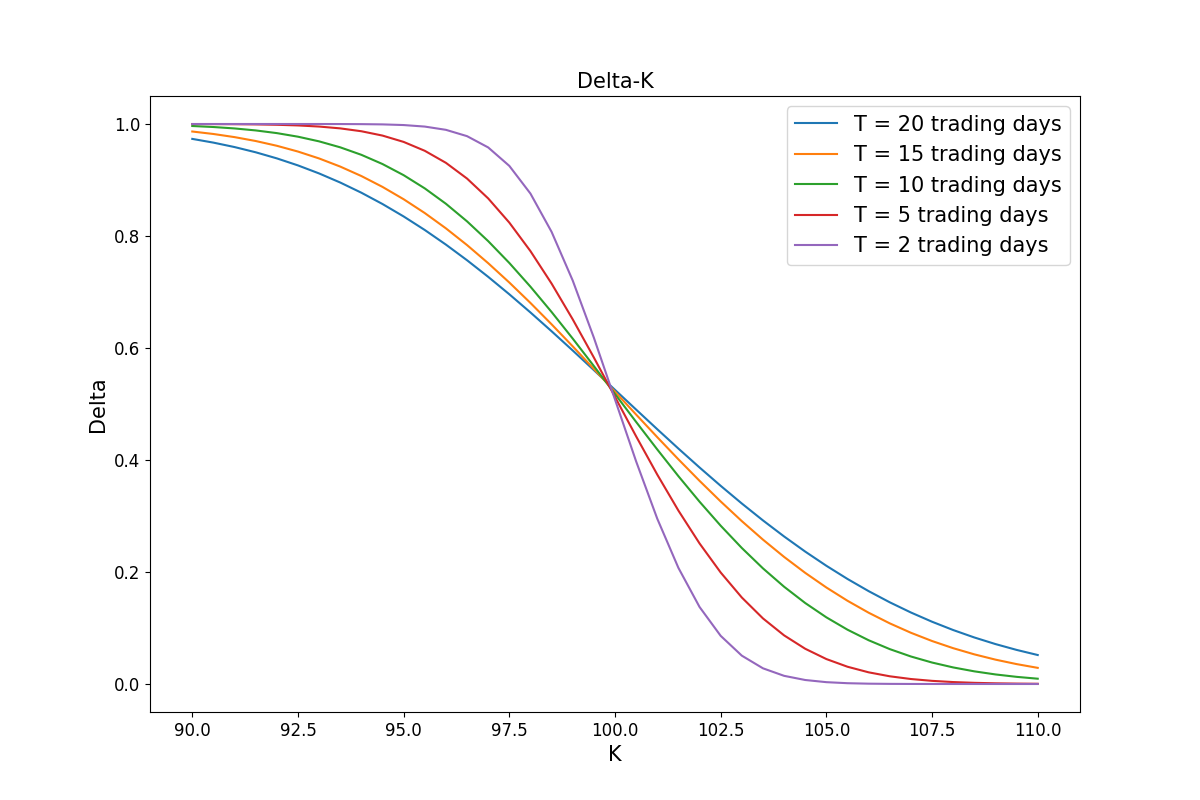
\includegraphics[width=12cm, height=8cm]{theory/delta_K.png}
  \caption[这里将出现在插图索引中]
    {看涨期权Delta与K和T的关系}
  \label{fig:delta_k}
\end{figure}

\begin{figure}[!htp]
  \centering
  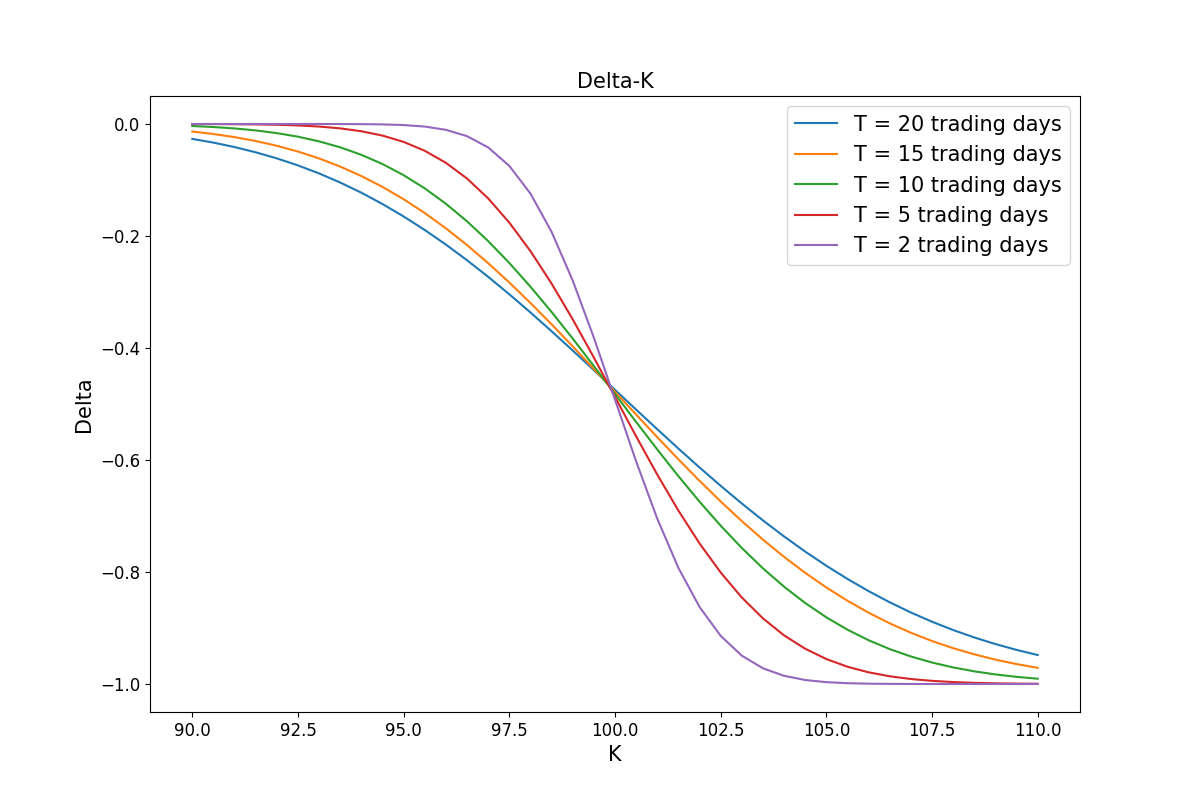
\includegraphics[width=12cm, height=8cm]{theory/put_delta_K.png}
  \caption[这里将出现在插图索引中]
    {看涨期权Delta与K和T的关系}
  \label{fig:put_delta_k}
\end{figure}

看涨期权的Delta值与行权价K和到期剩余时间T的关系如图\ref{fig:delta_k}所示,看跌期权的Delta值与行权价K和到期剩余时间T的关系如图\ref{fig:put_delta_k}所示。对于看涨期权来说,Delta始终为正,并且行权价K越高,Delta的绝对值越低;对于看跌期权来说,Delta始终为负,并且行权价K越高,Delta的绝对值越高,这其实可以从Delta的性质得到直观的理解。以看涨期权为例,Delta的计算公式为$N(d_1)$,与$N(d_2)$非常接近,而$N(d_2)$代表了在到期日标的价格达到K以上的概率,即看涨期权在到期日被行权的概率。因此,行权价K越高,看涨期权在到期日被行权的概率越低,Delta的绝对值越低。


\section{模拟方法}

在动态对冲研究中,模拟方法主要应用在资产价格路径的模拟上。关于资产价格路径的模拟,常用的有蒙特卡洛(Monte Carlo)方法和拟蒙特卡洛(Quasi-Monte Carlo)方法。蒙特卡洛方法是数值模拟中最为常用的方法,它实际上是这一类模拟方法的总称。本文所说的蒙特卡洛方法是一个相对狭义的概念,是指通过生成随机(random)或伪随机(pseudo-random)序列,模拟一个随机事件的可能情况,进而用频率来估计概率的方法。根据大数定律,若想有效地应用蒙特卡洛方法,需要较多的模拟的次数。在本文的研究中,我们并不直接考察每一次模拟的结果,而是对每一次的结果的一个函数进行求期望的操作,这一期望即为蒙特卡洛积分。设模拟次数为N,根据中心极限定理,蒙特卡洛积分的收敛速度为$O(N^{-\frac{1}{2}})$。蒙特卡洛的优势在于,其收敛速度独立于积分的维数。这一特点也使得其鲁棒性非常强,可以适用于很多高维的问题。然而,这一鲁棒性的代价是相对较慢的收敛速度。若要将误差的标准差大小的小数点向后移一位,需要将模拟次数提升为的100倍。

虽然蒙特卡洛方法鲁棒性较好,但是其对计算时间要求较高,因此本文最初希望可以找到一种收敛速度更快同时又不失鲁棒性的方法。我们考察了拟蒙特卡洛方法。拟蒙特卡洛方法使用低差异序列(low discrepancy sequence)进行模拟,经典的低差异序列包括Halton序列、Sobol序列和Faure序列。差异(discrepancy)是用来形容均匀性(uniformity)的,低差异序列比伪随机序列更接近均匀分布。与蒙特卡洛方法使用线性同余法等方法通过生成伪随机序列来试图模仿随机数的性质不同,低差异序列实际上是确定性的序列,并且其具有一定的自相关性来降低差异。因此拟蒙特卡洛方法只能用在蒙特卡罗积分问题上,使用其进行优化或单纯考察其模拟的结果是无意义的。拟蒙特卡洛模拟的收敛速度是$O((logN)^{d}N^{-1})$,其中d为模拟的维数。从这一收敛速度可以看出,当模拟次数N相对于维数d很大时,可以获得接近$O(N^{-1})$的收敛速度。然而,当d增长时,N需要以指数速度增长,以维持相应的收敛速度。如果N不足够大的话,拟蒙特卡洛模拟的收敛速度会慢于蒙特卡洛模拟的收敛速度。正如Caflisch(1998)指出的,高维性会很大程度上限制拟蒙特卡洛模拟的有效性。具体到本文的研究上,由于动态对冲是一个路径依赖的问题,因此其对应的维数即为标的资产价格路径模拟的频数,这一维数通常会很高(大于50)。在这样高维的模拟下,拟蒙特卡洛模拟效果将不如蒙特卡洛模拟。因此,在之后的研究中,本文将使用蒙特卡洛模拟生成资产价格序列。

当然,蒙特卡洛模拟可以通过方差减少技术来加快收敛速度,这一速度上的提高通常是通过减小$O(N^{-\frac{1}{2}})$项的系数,而并不会将速度提升一个量级,因此,对于这一技术,本文将不深入进行讨论,亦不会在应用中有所体现。关于拟蒙特卡洛模拟在高维情况下表现较差的问题,Wang和Sloan(2008)给出了一个解决方法,他们使用了一个新的计算差异的算法,使得拟蒙特卡洛方法在高维时的表现优于或至少不弱于蒙特卡洛方法。对于这一算法的细节、实现及应用,本文亦不进行讨论,而是将其作为未来可能的改进方向。

在确定了模拟使用的方法后,我们只是得到了生成参数为$(0,1)$的均匀分布的随机数的方式。获得了这一随机数后,可以使用正态分布的逆变换获得正态分布的随机数。之后,基于标的资产符合几何布朗运动的假设,生成价格序列。
